\documentclass[a4paper, 12pt]{article}
\usepackage{/Users/fgu/dev/projects/dotfiles/latex/paper}
\bibliography{/Users/fgu/dev/projects/dotfiles/latex/fabib}
\onehalfspacing

\newcommand{\figdir}{../../output/figures}
\newcommand{\tabdir}{../../output/tables}

\newcommand{\setc}{\mathcal{C}}
\newcommand{\setcp}{\mathcal{C}^{+}}
\newcommand{\setcz}{\mathcal{C}^{0}}
\newcommand{\regtabinfo}{Terms in brackets denote the upper and lower ends of a
95\% confidence interval. Standard errors are clustered at the user-level.} 


\title{\textbf{Spending profiles predict savings\footnote{We are grateful to
            Redzo Mujcic and and Zvi Safra for helpful comments. The research
            was supported by Economic and Social Research Council grant number
            ES/V004867/1. WBS ethics code: E-414-01-20.  Gunzinger: Warwick
Business School, fabian.gunzinger@warwick.ac.uk; Stewart: Warwick Business
School, neil.stewart@wbs.ac.uk.}}}

\author{Fabian Gunzinger \and Neil Stewart}

\date{\today}


% conventions
% users: individuals throughout (not people or users or something else!)



\begin{document}

\maketitle

% % !TEX root = ../entropy.tex

\begin{abstract}
    ...
\end{abstract}


\tableofcontents
\newpage

% !TEX root = ../entropy.tex

\section{Introduction}%
\label{sec:introduction}

This paper documents variations in spending profiles and payments into
emergency savings for a large set of users of a financial management app
and shows that spending profiles predict emergency savings.

We define emergency savings as inflows into savings accounts. These savings
will be made up of savings for particular goals -- a new car, a holiday, a
wedding -- and savings directed towards building up a buffer for financial
emergencies. Because in our data we cannot distinguish between these two cases,
we refer to all of them as emergency savings.\footnote{MDB allows users to
    create custom tags and some users use them to indicate the intended use for
    their savings transactions (e.g. ``wedding'', ``holidays''). But only a very
small number of transactions have such tags, and we do not pursue this
further.} These short-term savings are distinct from long-term savings aimed to
build up funds for retirement, either through individually owned pension and
investment vehicles or employer-linked pension schemes. Both kinds of saving
are important for financial well-being, yet while there is a large literature
on pension savings, little is known about how people save for the
short-term.\footnote{Well-documented behavioural biases that help explain
    undersaving for pensions are, among others, present bias
    \citep{laibson1997golden, laibson2019intertemporal}, inertia
    \citep{madrian2001power}, over-extrapolation \citep{choi2009reinforcement},
    and limited self-control and willpower \citep{thaler1981economic,
    benhabib2005modeling, fudenberg2006dual, loewenstein2004animal,
gul2001temptation}. One danger of viewing low savings mainly as a result of
behavioural biases is that while these biases likely do play some role and
designing environments and tools to help correct them are thus part of the
solution, it is at least conceivable that this is an area where the focus on
behaviour-level solutions distracts from an effort to find more effective
society-level solutions, a danger inherent in behavioural science research
convincingly highlighted in \citet{chater2022frame}: if the main problem is
that many people are unable to earn enough to save, then the effectiveness of
helping them manage their low incomes more effectively pales in comparison with
efforts to help them earn more.}

Studying the determinants of emergency savings is important because around a
quarter of adults in the UK and the US are unable to cover irregular expenses
like car and medical bills: In the UK, 25 percent of adults would be unable to
cover an unexpected bill of \pounds300 \citep{philipps2021supporting}, while in
the US, about 30 percent would be unable to cover a \$400 bill
\citep{fed2022economic}. Similarly, resarch in the UK has shown that having
\pounds1000 in savings reduces by more than half a household's chances of
falling into debt that leads to financial problems
\citep{philipps2021supporting}.


Studying spending profiles is of interest because:
\begin{itemize}

    \item Our understanding of how people spend their money is based on survey
        data.

    \item Large-scale transaction-level data offers the possibility to study
        spending behaviour based on real-time data that are automatically
        collected for a large number of users. Such data has only become
        available ver recently and have not, thus far, been used to investigate
        systematically how people spend their money.

    \item Research in psychology suggests that disorder is maladaptive and
        associated with a range of negative outcomes such as impaired executive
        function \citep{vernon2016predictors}, lower cognitive inhibition
        \citep{mittal2015cognitive}, and activation of anxiety-related neural
        circuits \citep{hirsh2012psychological}. In the study of human
        behaviour, more chaotic behaviour has been found to predict the a
        higher number of visits to and higher spend in supermarkets
        \citep{guidotti2015behavioral}, higher calorie intake
        \citep{skatova2019those} and financial distress
        \citep{muggleton2020evidence}.

\end{itemize}


We hypothesise that less predictable spending patterns are associated with a
lower probability for making payments into emergency savings accounts. Possible
channels:
\begin{itemize}
    \item Disorder (personal life or environment): leads to more impulsive
        shopping behaviour and makes forgetting to save more likely.

    \item Scarcity: life challenges focus attention away from deliberate
        shopping, causing hore impulse purchases, and make fortetting to save
        more likely.
\end{itemize}



What we do: 
\begin{itemize}

    \item Systematically documenting emergency savings patterns.

    \item Systematically documenting variation in spending profiles.

    \item Showing that unpredictability in spending profiles is
        associated with lower emergency savings.

\end{itemize}


Contribution to literatures:
\begin{itemize}

    \item Understanding emergency savings behaivour (nest, aspen
        reports), \citep{sabat2019rules} for sources on short-term savings
        literature, \citet{colby2013savings} for lit on savings goals.  See
        \citet{colby2013savings} has useful literature review on short-term
        savings and suggests that subgoals can increase willingness to forego
        short-amounts in the present because they move the reference point in a
        prospect-theory framework. \citet{philipps2021supporting} present
        results from an employer-linked initiative that offers employees to
        have a portion of their salary automatically transferred into a savings
        pot. Policy literature: \citep{can2019improving,cfpb2017financial,
        mps2018building}. Older literature:Savings lit:
        \citet{lunt1991psychological, oaten2007improvements}

    \item Understanding effect of behavioural entropy - eliciting
        useful personality characteristics from large-scale data.

    \item Use of high-frequency transaction data (itself a
        sub-literature of use of newly available large-scale datasets).

\end{itemize}



% !TEX root = ../entropy.tex

\section{Methods}%
\label{sec:methods}



\subsection{Model specification}%
\label{sub:model_specification}



\begin{equation}
    s_{i,t} = \alpha_i + \lambda_t + \beta H_{i,t} + \zeta X_{i,t} + \epsilon_{i,t}
\end{equation}

$s_{i,t}$ is individual $i$'s savings rate in month $t$, calculated as the
total inflow of funds in month $t$ into all savings accounts held by $i$,
divided by $i$'s estimated monthly income.

The vector of control variables, $X_{i,t}$, contains the monthly spend for each
spending category, total monthly spend across all categories, and annual income.






% !TEX root = ../entropy.tex

\section{Spending profiles}%
\label{sec:spending_profiles}

% Figure~\ref{fig:spending}
% \begin{figure}[H]
%     \center \newcommand\width{\textwidth} \caption{Spending behaviour}
%     \label{fig:spending}
%     \includegraphics[width=\width]{\figdir/spending.png}
% \end{figure}





% !TEX root = ../entropy.tex

\section{Savings patterns}%
\label{sec:savings_patterns}

\begin{figure}[H]
    \center \newcommand\width{\textwidth} \caption{Savings behaviour}
    \label{fig:savings}
    \includegraphics[width=\width]{\figdir/savings.png}
\end{figure}



% !TEX root = ../entropy.tex

\section{Spending profiles predict emergency savings}%
\label{sec:results}

Table~\ref{tab:reg_has_inflows_main} shows the effect of entropy on the
probability of having emergency savings. Columns (1)-(3) show results for
unsmoothed entropy based on 9 categories, 48 categories, and merchant names,
respectively. Columns (4)-(6) results for smoothed entropy based on the same
variables. All models include user and year-month fixed effects, and standard
errors are clustered at the user-level. Confidence intervals are shown in
brakets.

\input{\tabdir/reg_has_inflows_main.tex}

Results for unsmoothed entropy suggest that a one unit increase in entropy is
associated with an increase in the probability of a user making at least one
transfer into their savings accounts of between 1.5 and 2.7 percentage points
-- an effect up to two times larger than that of a \pounds1000 increase in
monthly income.

Conversely, the effect for unsmooth entropy is smaller in magnitude but runs in
the reverse direction: a one-unit increase in the smoothed entropy score is
associated with a reduction in the probability of transferring money into
savings account of between 0.4 and 1.6 percentage points -- an effect that, in
absolute magnitude, is about equal to that of a \pounds1000 increase in monthly
income.

Overall, then, the effect of entropy in spending profiles is statistically and
economically significant, and robust across different definitions. In other
words, the scores seem to pick up a feature of the spending distribution that
is predictive of savings behaviour.

But how can we account for the opposite sign for smoothed and unsmoothed
entropy scores? We don't have the answer to this yet... 


\subsection{Effect of financial resilience}%
\label{sub:effect_of_financial_resilience}




If we think that it is scarcity that causes the relationship between
unpredictable spending behaviour and savings, then we would expect the effect
to be strongest for people with the lowest incomes, since they are more prone
to face financial shocks they find difficult to meet. The results below support
such an interpretation: the effect of both unsmoothed and smoothed entropy on
the probability of making a savings transaction is largest in magnitude for
users in the first income quintile.

In these regressions, we do not control for whether a user has income in in a
given month, since for all but the group in the first income quintile, this
will always be the case.


\begin{table}[htbp]
   \centering
   \tiny
   \begin{threeparttable}[b]
      \caption{\label{tab:reg_has_inflows_entropy_tag_spend_z_inc_quint} Effect of entropy on P(has savings) by income quintile}
      \begin{tabular}{lccccc}
         \tabularnewline \midrule \midrule
         Model:             & (1)             & (2)             & (3)            & (4)            & (5)\\  
         Income quintile:   & 1               & 2               & 3              & 4              & 5 \\   
         \midrule
         \emph{Variables}\\
         Entropy (48 cats)  & 0.033$^{***}$   & 0.019$^{***}$   & 0.017$^{***}$  & 0.016$^{***}$  & 0.018$^{***}$\\   
                            & [0.028; 0.039]  & [0.013; 0.025]  & [0.011; 0.023] & [0.010; 0.022] & [0.012; 0.025]\\   
         Month spend        & 0.010$^{***}$   & 0.007$^{***}$   & 0.008$^{***}$  & 0.007$^{***}$  & 0.006$^{***}$\\   
                            & [0.009; 0.011]  & [0.006; 0.008]  & [0.006; 0.009] & [0.006; 0.008] & [0.005; 0.007]\\   
         Month income       & 0.015$^{***}$   & 0.010$^{***}$   & 0.012$^{***}$  & 0.013$^{***}$  & 0.008$^{***}$\\   
                            & [0.012; 0.019]  & [0.004; 0.017]  & [0.005; 0.019] & [0.008; 0.019] & [0.007; 0.010]\\   
         Income variability & -0.000          & 0.001           & 0.002$^{***}$  & 0.001$^{**}$   & -0.000\\   
                            & [-0.001; 0.001] & [-0.000; 0.002] & [0.001; 0.004] & [0.000; 0.002] & [-0.001; 0.001]\\   
         \midrule
         \emph{Fixed-effects}\\
         User               & Yes             & Yes             & Yes            & Yes            & Yes\\  
         Year-month         & Yes             & Yes             & Yes            & Yes            & Yes\\  
         \midrule
         \emph{Fit statistics}\\
         Observations       & 223,462         & 215,151         & 208,417        & 201,319        & 195,378\\  
         R$^2$              & 0.59138         & 0.58949         & 0.58354        & 0.58212        & 0.57162\\  
         Within R$^2$       & 0.00535         & 0.00180         & 0.00211        & 0.00191        & 0.00271\\  
         \midrule \midrule
         \multicolumn{6}{l}{\emph{Clustered (User) co-variance matrix, 95\% confidence intervals in brackets}}\\
         \multicolumn{6}{l}{\emph{Signif. Codes: ***: 0.01, **: 0.05, *: 0.1}}\\
      \end{tabular}
   \end{threeparttable}
\end{table}



\input{\tabdir/reg_has_inflows_entropy_tag_spend_sz_inc_quint.tex}


\begin{table}[htbp]
   \centering
   \tiny
   \begin{threeparttable}[b]
      \caption{\label{tab:reg_has_inflows_entropy_tag_spend_z_inc_var_quint} Effect of entropy on P(has savings) by income variability quintile}
      \begin{tabular}{lccccc}
         \tabularnewline \midrule \midrule
         Model:                       & (1)             & (2)            & (3)             & (4)             & (5)\\  
         Income variability quintile: & 1               & 2              & 3               & 4               & 5 \\   
         \midrule
         \emph{Variables}\\
         Entropy (48 cats)            & 0.020$^{***}$   & 0.014$^{***}$  & 0.022$^{***}$   & 0.028$^{***}$   & 0.021$^{***}$\\   
                                      & [0.014; 0.026]  & [0.008; 0.020] & [0.016; 0.028]  & [0.022; 0.034]  & [0.015; 0.027]\\   
         Month spend                  & 0.008$^{***}$   & 0.008$^{***}$  & 0.007$^{***}$   & 0.007$^{***}$   & 0.007$^{***}$\\   
                                      & [0.007; 0.009]  & [0.007; 0.009] & [0.006; 0.008]  & [0.006; 0.008]  & [0.006; 0.008]\\   
         Month income                 & 0.014$^{***}$   & 0.010$^{***}$  & 0.011$^{***}$   & 0.010$^{***}$   & 0.010$^{***}$\\   
                                      & [0.011; 0.017]  & [0.008; 0.012] & [0.010; 0.013]  & [0.009; 0.012]  & [0.009; 0.011]\\   
         Has income in month          & 0.092$^{***}$   & 0.076$^{***}$  & 0.064$^{***}$   & 0.055$^{***}$   & 0.067$^{***}$\\   
                                      & [0.073; 0.111]  & [0.056; 0.095] & [0.047; 0.081]  & [0.040; 0.070]  & [0.053; 0.081]\\   
         Income variability           & -0.001          & 0.006$^{**}$   & -0.000          & 0.000           & -0.004$^{**}$\\   
                                      & [-0.003; 0.001] & [0.001; 0.011] & [-0.004; 0.003] & [-0.001; 0.002] & [-0.007; -0.001]\\   
         \midrule
         \emph{Fixed-effects}\\
         User                         & Yes             & Yes            & Yes             & Yes             & Yes\\  
         Year-month                   & Yes             & Yes            & Yes             & Yes             & Yes\\  
         \midrule
         \emph{Fit statistics}\\
         Observations                 & 223,462         & 215,151        & 208,417         & 201,319         & 195,378\\  
         R$^2$                        & 0.61166         & 0.59951        & 0.59062         & 0.59379         & 0.63519\\  
         Within R$^2$                 & 0.00558         & 0.00398        & 0.00484         & 0.00579         & 0.00781\\  
         \midrule \midrule
         \multicolumn{6}{l}{\emph{Clustered (User) co-variance matrix, 95\% confidence intervals in brackets}}\\
         \multicolumn{6}{l}{\emph{Signif. Codes: ***: 0.01, **: 0.05, *: 0.1}}\\
      \end{tabular}
   \end{threeparttable}
\end{table}




\begin{table}[htbp]
   \centering
   \tiny
   \begin{threeparttable}[b]
      \caption{\label{tab:reg_has_inflows_entropy_tag_spend_sz_inc_var_quint} Effect of entropy on P(has savings) by income variability quintile}
      \begin{tabular}{lccccc}
         \tabularnewline \midrule \midrule
         Model:                       & (1)              & (2)              & (3)              & (4)              & (5)\\  
         Income variability quintile: & 1                & 2                & 3                & 4                & 5 \\   
         \midrule
         \emph{Variables}\\
         Entropy (48 cats, smooth)    & -0.019$^{***}$   & -0.020$^{***}$   & -0.017$^{***}$   & -0.022$^{***}$   & -0.024$^{***}$\\   
                                      & [-0.024; -0.015] & [-0.024; -0.016] & [-0.021; -0.013] & [-0.026; -0.018] & [-0.028; -0.019]\\   
         Month spend                  & 0.007$^{***}$    & 0.007$^{***}$    & 0.006$^{***}$    & 0.006$^{***}$    & 0.006$^{***}$\\   
                                      & [0.006; 0.008]   & [0.006; 0.008]   & [0.005; 0.008]   & [0.005; 0.007]   & [0.005; 0.007]\\   
         Month income                 & 0.014$^{***}$    & 0.010$^{***}$    & 0.011$^{***}$    & 0.010$^{***}$    & 0.010$^{***}$\\   
                                      & [0.011; 0.017]   & [0.008; 0.012]   & [0.009; 0.013]   & [0.009; 0.012]   & [0.009; 0.011]\\   
         Has income in month          & 0.093$^{***}$    & 0.075$^{***}$    & 0.064$^{***}$    & 0.056$^{***}$    & 0.066$^{***}$\\   
                                      & [0.074; 0.112]   & [0.055; 0.094]   & [0.047; 0.081]   & [0.040; 0.071]   & [0.052; 0.081]\\   
         Income variability           & -0.001           & 0.005$^{**}$     & -0.000           & 0.000            & -0.004$^{**}$\\   
                                      & [-0.003; 0.001]  & [0.001; 0.010]   & [-0.004; 0.003]  & [-0.001; 0.002]  & [-0.006; -0.001]\\   
         \midrule
         \emph{Fixed-effects}\\
         User                         & Yes              & Yes              & Yes              & Yes              & Yes\\  
         Year-month                   & Yes              & Yes              & Yes              & Yes              & Yes\\  
         \midrule
         \emph{Fit statistics}\\
         Observations                 & 223,462          & 215,151          & 208,417          & 201,319          & 195,378\\  
         R$^2$                        & 0.61181          & 0.59979          & 0.59070          & 0.59394          & 0.63550\\  
         Within R$^2$                 & 0.00597          & 0.00466          & 0.00502          & 0.00614          & 0.00864\\  
         \midrule \midrule
         \multicolumn{6}{l}{\emph{Clustered (User) co-variance matrix, 95\% confidence intervals in brackets}}\\
         \multicolumn{6}{l}{\emph{Signif. Codes: ***: 0.01, **: 0.05, *: 0.1}}\\
      \end{tabular}
   \end{threeparttable}
\end{table}







% !TEX root = ../entropy.tex

\section{Discussion}%
\label{sec:discussion}

\edit{Ignore this section for now. Below are just notes.}
There are a number of alternative ways to characterise spend profiles. We could
calculate profiles based on the distribution of transaction values rather than
counts. We could also calculate profiles based on inter-temporal rather than
intra-temporal distributions, focusing on consistency of purchasing behaviour
over time rather than on predictability at any given time
\citep{krumme2013predictability}. Further, we could focus on time-based rather
than category-based measures, focusing, for instance, on whether purchases of
the same type tend to occur on the same day of the week
\citep{guidotti2015behavioral}. Finally, one could also create composite
measures based on principal component analysis, an approach used in
\citet{eagle2010network}. We leave these extensions for future research.



\newpage
\printbibliography
\newpage

\appendix

% !TEX root = ../entropy.tex

\section{Interpreting entropy}%
\label{sec:interpreting_entropy}




% !TEX root = ../entropy.tex

\section{Additional results}%
\label{sec:additional_results}

\subsection{Endogeneity}%
\label{sub:endogeneity}

As discussed in Section~\ref{sub:estimation}, one concern one might have about
our results in Section~\ref{sec:results} is reverse causality:
transferring money into savings accounts might change the distribution of spend
categories and thus change entropy. As noted previously, this is not a major
concern because of the way we calculate savings and spend profiles: savings are
calculated as the sum of inflows into savings accounts, while spend profiles
are based on the classification of spend transactions in current accounts, and
transfers from current to savings accounts are labelled as such and not treated
as spend transactions.

However, because transaction labelling is imperfect, it is possible that some
transfers are misclassified as spends and included in the calculation of
entropy scores. One way to deal with this is to lag entropy scores by one
period. Table~\ref{tab:main_lag} presents results similar to the main
results in the main text, but using entropy lagged by one year-month period as
the independent variable of interest. We can see that the results are very
similar to thos presented above.

\def\yvars{has_inflows}
\foreach \y in \yvars {
    \begin{table}[ht]
    \centering\tiny
    \caption{Effect of lagged entropy on P(savings transactions)}
    \label{tab:main_lag}
    \input{\tabdir/reg_\y_lag.tex}
    \tabnote{.95\textwidth}{Results from estimating Equation~\ref{equ:model}. The
        dependent variable in all columns is a dummy variable indicating whether a
        user made at least one transaction into any of their savings accounts in a
    given period. Entropy variables are lagged by one period. \regtabinfo}
    \end{table}
}


\subsection{Entropy components}%
\label{sub:entropy_components}

\begin{figure}[ht]
    \centering 
    \caption{Correlation of entropy with its components}
    \label{fig:entropy_components}
    \includegraphics[width=.32\textwidth]{\figdir/scatter_entropy_nunique_tag_spend.pdf}
    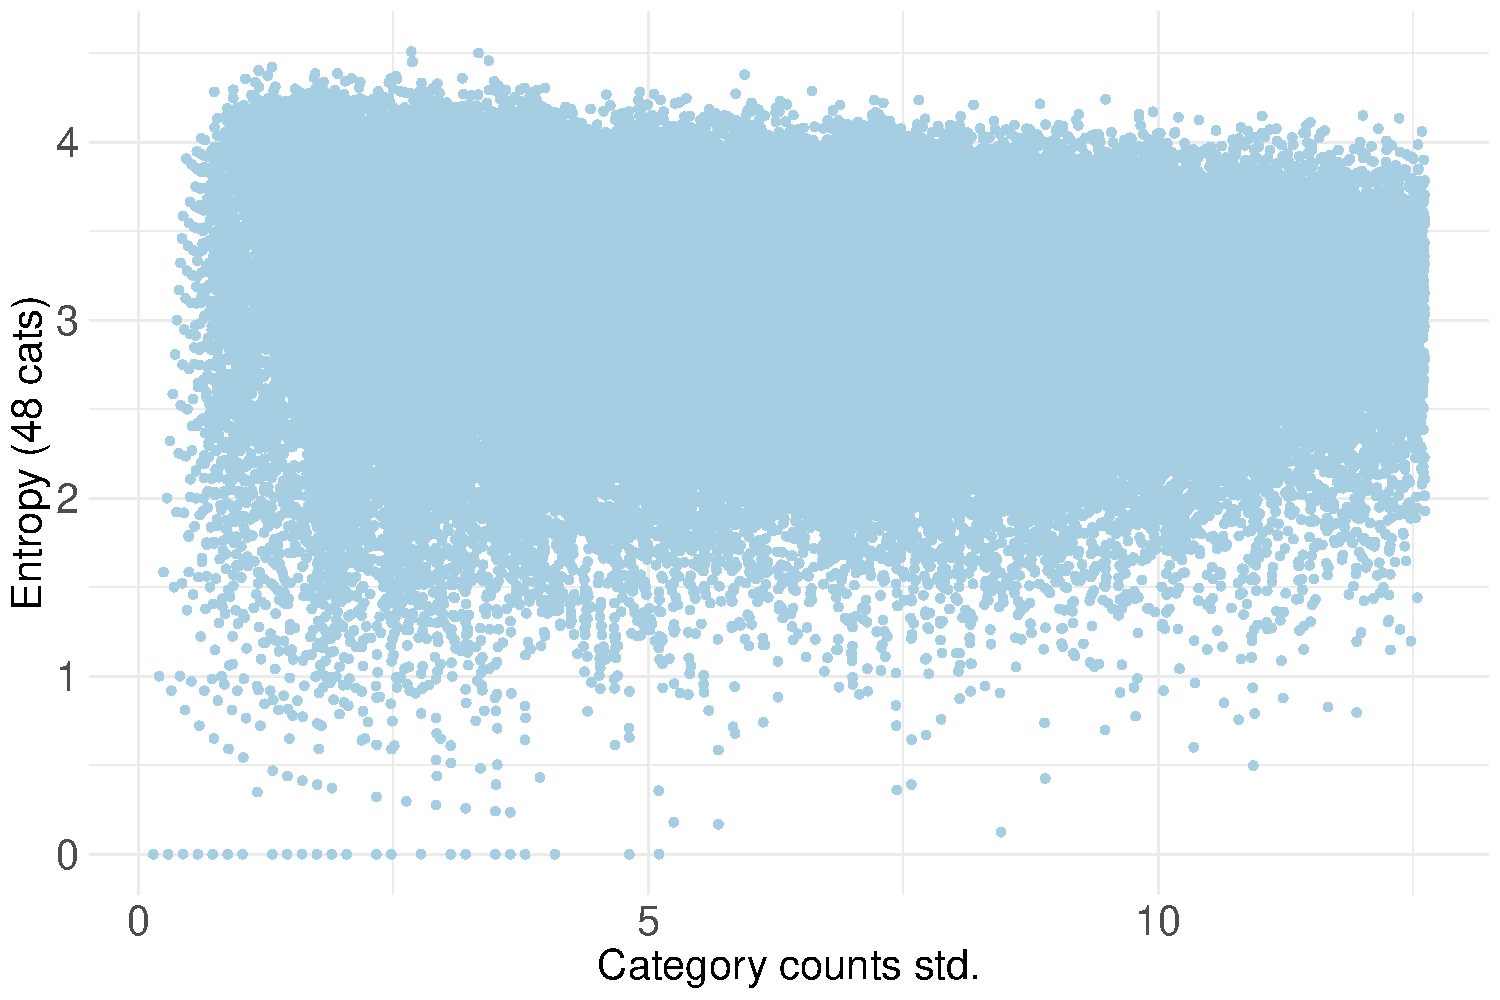
\includegraphics[width=.32\textwidth]{\figdir/scatter_entropy_std_tag_spend.pdf}
    \includegraphics[width=.32\textwidth]{\figdir/scatter_entropy_txns_count_spend.pdf}
    \fignote{\textwidth}{Correlation of 48-categories-based unsmoothed entropy
    with its three main components: the number of unique spending categories
with positive frequency counts (left), the standard deviation of those
frequency counts (middle), and the number of total spend transactions (left).}
\end{figure}

Figure~\ref{fig:entropy_components} shows the empirical relationship with our
48-categories-based unsmoothed entropy variable and these three
components.\footnote{To highlight the main features of the relationships we
have trimmed the component values at the 95th percentile.} We can see that for
the values we observe in the dataset, entropy increases monotonically in the
number of unique spending categories with positive frequency counts, has no
clear relationship with the standard deviation of those counts, and increases
in the number of total spending transactions up to about 175 transaction,
before being increasingly determined by other elements thereafter.


\subsection{Effect of smothing on entropy (by number of spend quintile)}%
\label{sub:effect_of_smothing_on_entropy_by_number_of_spend_quintile_}

\begin{figure}[ht]
    \centering 
    \caption{Effect of smoothing on entropy}
    \label{fig:scatter_facets_txns_count_spend_q}
    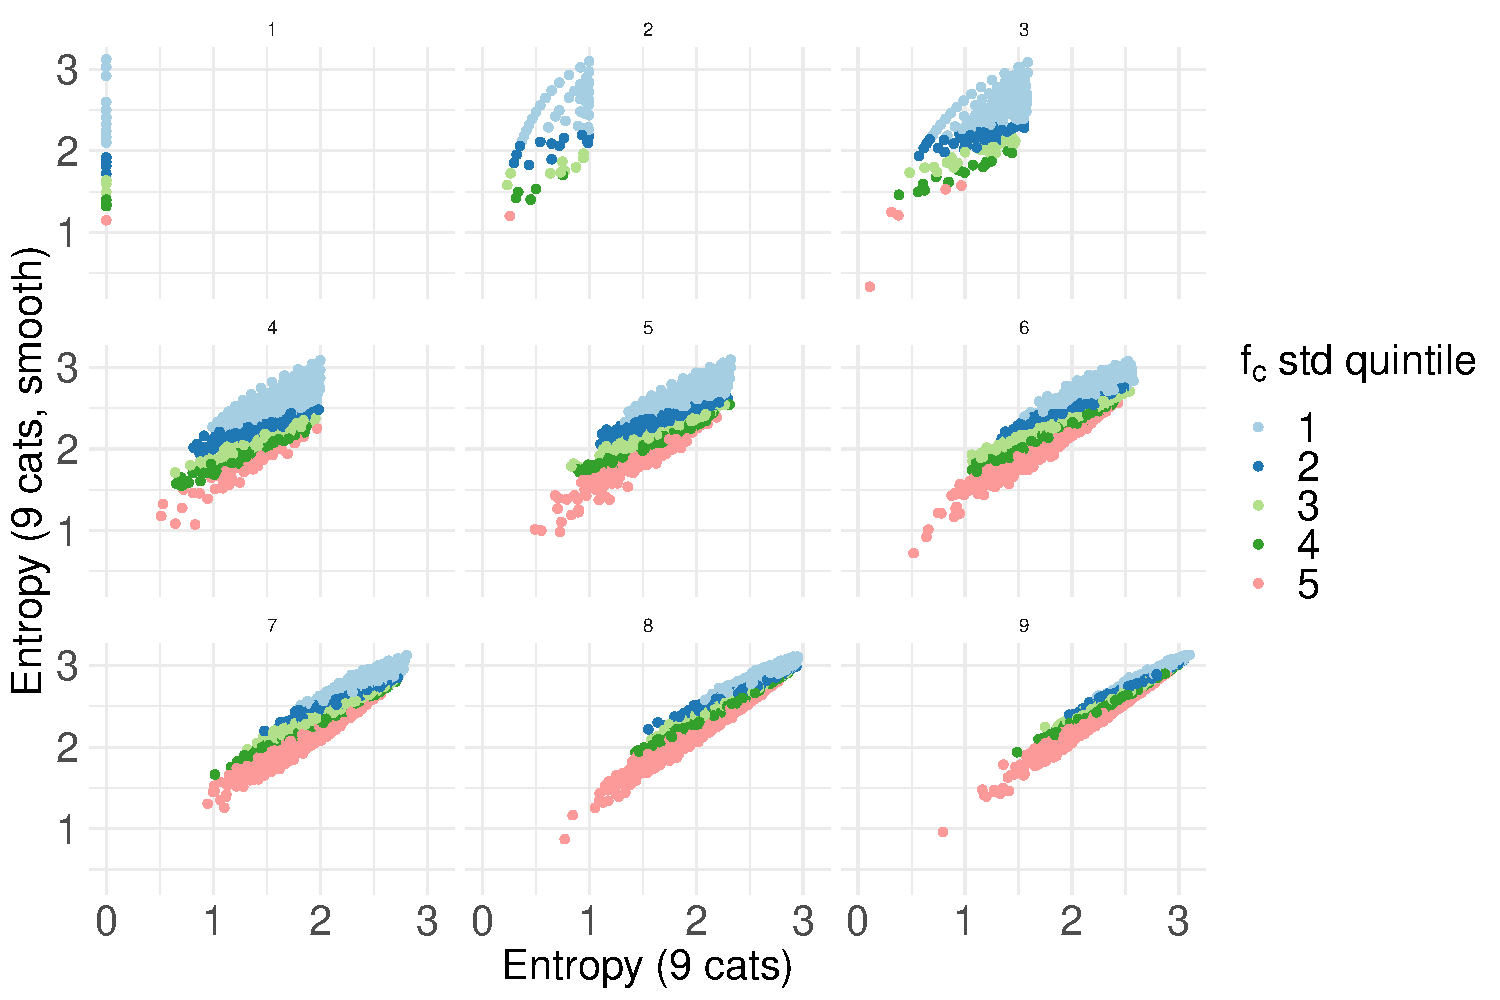
\includegraphics[width=\textwidth]{\figdir/scatter_facet_std_tag_q.pdf}
    \fignote{\textwidth}{Percentile ranks of 9-category-based unsmoothed and
    smoothed entropy separated by the number of categories with positive
frequency counts. White reference lines indicate equal percentile ranks.
Colours indicate the quintile of the total number of spending transactions.}
\end{figure}



\end{document}
